In recent years rehabilitation medicine, and prosthetics in
particular, has benefited from the advances in mechatronics, a field
which has so far pertained to robotics. This synergy is driving
rehabilitation medicine to a scenario in which an amputee's life will
be better, when more dexterous and controllable prostheses will make
it to the market. The paradigmatic example is represented by the
recent commercialisation of Touch Bionics's i-LIMB prosthetic hand
\cite{ilimb}, which is lightweight, long-running, it has five fingers
and five Degrees-Of-Freedom (DOFs --- one per finger, see Figure
\ref{fig:hands} $(a)$). (At the time of writing, a few hundreds i-LIMBs
have been implanted and sold.)

\begin{figure}
  \begin{tabular}{ccc}
    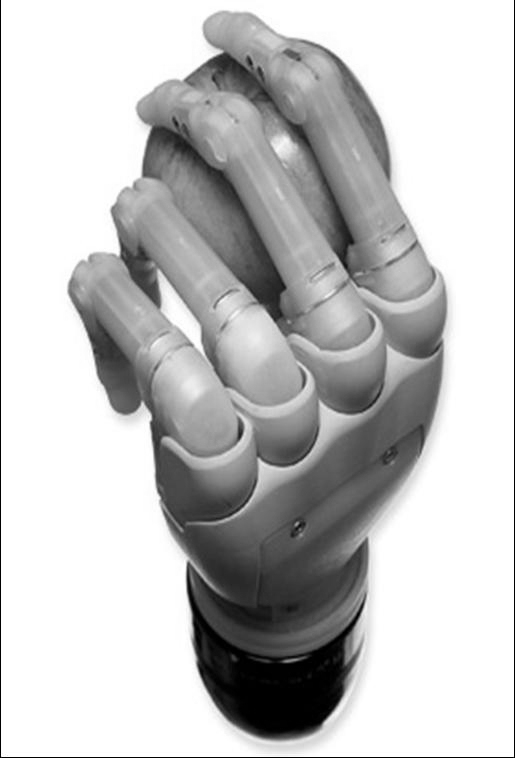
\includegraphics[width=0.14\textwidth]{figs/hands_TB.jpg} &
    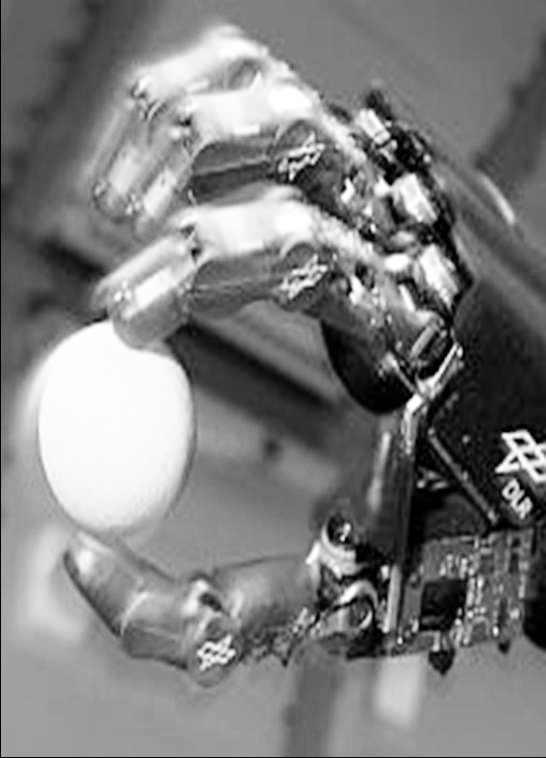
\includegraphics[width=0.14\textwidth]{figs/hands_DLRII.jpg} &
    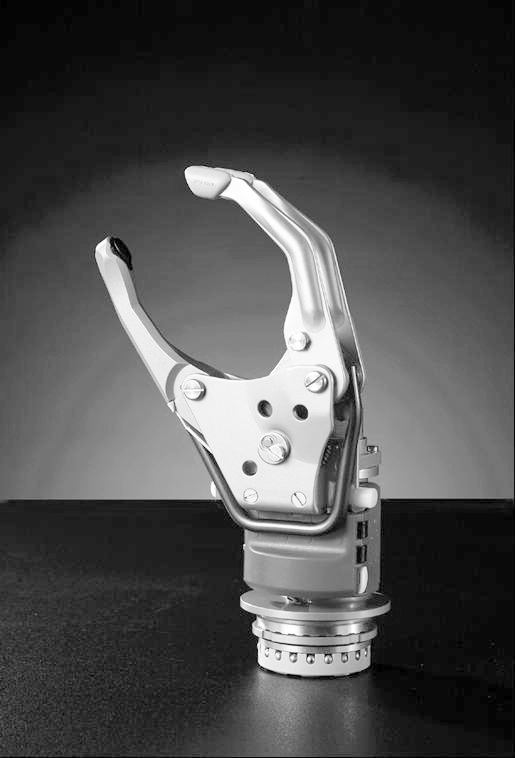
\includegraphics[width=0.14\textwidth]{figs/hands_OB.jpg} \\
    $(a)$ & $(b)$ & $(c)$
  \end{tabular}
  \caption{$(a)$ Touch Bionics's i-LIMB prosthetic hand (reproduced
    from \cite{ilimb}; $(b)$ the DLR-II mechanical hand; $(c)$ Otto
    Bock's SensorHand Speed (reproduced from \cite{sensorhand}).}
  \label{fig:hands}
\end{figure}

The dexterity of this prosthesis is very high, though still far from
the best non-prosthetic robot hand prototypes (e.g., the DLR-II hand,
see \cite{Hua2006} and Figure \ref{fig:hands} $(b)$). In fact, it
represents a real breakthrough with respect to the state-of-the-art
commercial prostheses, namely Otto Bock's SensorHand Speed (see Figure
\ref{fig:hands} $(c)$), which has one open/close DOF. Notice, anyway,
that both prostheses still allow for no control of the \emph{force}
required by the patient.

In fact, control is, in general, far from optimal. The most widely
used control device nowadays is surface electromyography (EMG), a
cheap, non-invasive technique by which surface electrodes gather from
the patient's stump skin the (residual) muscle activation potentials
(see, e.g., \cite{deluca}); these potentials are then somehow
translated to motor commands. The current EMG-based strategies employ
large muscles, such as the wrist flexor and extensor, to control one
or, at best, two DOFs (e.g., opening and closing of the Otto Bock's
claw). This means that controlling the prosthesis is highly
non-natural, and implies a long training time for the patient, that
is, the patient must learn how to order the hand what she/he wants it
to do.

Even a dexterous hand prosthesis as the i-LIMB cannot be controlled in
a fine and natural way; it uses two EMG electrodes in combination, to
produce a set of predefined grasp shapes; and the force involved in
the grasp is not controlled. Most of the adaptability is left to the
compliance of the hand itself. Notice that \emph{force control} is a
paramount requirement in Daily-Life Activities (DLA): picture the
possibility of holding an egg without breaking it, or holding a hammer
without letting it slip.

Indeed, as more advanced hand prostheses appear on the market, there
is a strong demand for \emph{accurate control strategies}. This paper
fits in this line of research, showing that plain, old-fashioned EMG,
together with \emph{machine learning} techniques, can be used in a
radically better way to control a dexterous hand prosthesis. In
\cite{2008.ICRA,2008.BioCyb} we have shown that ten EMG electrodes
could enable a healthy human subject to force-control a dexterous
mechanical hand such as the DLR-II hand. Here we carry on the
analysis, extending it to $10$ healthy subjects and showing that the
same excellent results are obtained, regardless of the subject
involved; moreover, we relax the highly controlled conditions of the
previous experiment (the subject would keep her/his arm and body
posture rigorously relaxed and still) and show that the same
technique, applied to subjects who can freely move, walk, sit, raise
and lower their arms and pronate/supinate their forearms, obtains only
slightly worse results, which would most likely become optimal in an
online environment.

Our research aims at realising \emph{adaptive prosthetics}, that is,
the possibility for the prosthesis to adapt to the patient's needs and
style: so far, it is the patient that has to adapt to the prosthesis,
and learn how to use it. In our vision, the patient and the prosthesis
are involved in a \emph{reciprocal learning} loop. The result is that
the patient needs less time to correctly use the prosthesis, and also
that she/he can use it in a finer way, more suited to real DLAs. The
results presented in this paper show that this is possible. The final
question remains of whether an
\emph{amputee} can do the same; some initial results seem to indicate
that the answer is positive (see the ``Discussion and conclusions''
section for more details).

The paper is structured as follows: Section \ref{sec:m&ms} introduces
the materials and methods used for the experiments; Section
\ref{sec:exp} presents a detailed analysis of the gathered data, and
the results of it; lastly, in Section \ref{sec:discussion} we discuss
the results and draw a few conclusions.
